\documentclass[a4paper]{book}
\usepackage{a4wide}
\usepackage{makeidx}
\usepackage{graphicx}
\usepackage{multicol}
\usepackage{float}
\usepackage{listings}
\usepackage{color}
\usepackage{textcomp}
\usepackage{alltt}
\usepackage{times}
\usepackage{ifpdf}
\ifpdf
\usepackage[pdftex,
            pagebackref=true,
            colorlinks=true,
            linkcolor=blue,
            unicode
           ]{hyperref}
\else
\usepackage[ps2pdf,
            pagebackref=true,
            colorlinks=true,
            linkcolor=blue,
            unicode
           ]{hyperref}
\usepackage{pspicture}
\fi
\usepackage[utf8]{inputenc}
\usepackage{doxygen}
\lstset{language=C++,inputencoding=utf8,basicstyle=\footnotesize,breaklines=true,breakatwhitespace=true,tabsize=8,numbers=left }
\makeindex
\setcounter{tocdepth}{3}
\renewcommand{\footrulewidth}{0.4pt}
\begin{document}
\hypersetup{pageanchor=false}
\begin{titlepage}
\vspace*{7cm}
\begin{center}
{\Large BV Creator }\\
\vspace*{1cm}
{\large Generated by Doxygen 1.6.2}\\
\vspace*{0.5cm}
{\small Sat Jan 23 01:44:57 2010}\\
\end{center}
\end{titlepage}
\clearemptydoublepage
\pagenumbering{roman}
\tableofcontents
\clearemptydoublepage
\pagenumbering{arabic}
\hypersetup{pageanchor=true}
\chapter{Class Index}
\section{Class Hierarchy}
This inheritance list is sorted roughly, but not completely, alphabetically:\begin{DoxyCompactList}
\item \contentsline{section}{Controller}{\pageref{class_controller}}{}
\item \contentsline{section}{EnvironmentDrawWindow}{\pageref{class_environment_draw_window}}{}
\item \contentsline{section}{FileChooser}{\pageref{class_file_chooser}}{}
\item \contentsline{section}{LineSegment}{\pageref{class_line_segment}}{}
\begin{DoxyCompactList}
\item \contentsline{section}{Actuator}{\pageref{class_actuator}}{}
\end{DoxyCompactList}
\item \contentsline{section}{Point2D}{\pageref{class_point2_d}}{}
\item \contentsline{section}{Shape}{\pageref{class_shape}}{}
\item \contentsline{section}{VehicleDrawWindow}{\pageref{class_vehicle_draw_window}}{}
\item \contentsline{section}{VehicleModel}{\pageref{class_vehicle_model}}{}
\end{DoxyCompactList}

\chapter{Class Index}
\section{Class List}
Here are the classes, structs, unions and interfaces with brief descriptions:\begin{DoxyCompactList}
\item\contentsline{section}{\hyperlink{class_actuator}{Actuator} }{\pageref{class_actuator}}{}
\item\contentsline{section}{\hyperlink{class_controller}{Controller} }{\pageref{class_controller}}{}
\item\contentsline{section}{\hyperlink{class_environment_draw_window}{EnvironmentDrawWindow} }{\pageref{class_environment_draw_window}}{}
\item\contentsline{section}{\hyperlink{class_file_chooser}{FileChooser} }{\pageref{class_file_chooser}}{}
\item\contentsline{section}{\hyperlink{class_line_segment}{LineSegment} }{\pageref{class_line_segment}}{}
\item\contentsline{section}{\hyperlink{class_point2_d}{Point2D} }{\pageref{class_point2_d}}{}
\item\contentsline{section}{\hyperlink{class_shape}{Shape} }{\pageref{class_shape}}{}
\item\contentsline{section}{\hyperlink{class_vehicle_draw_window}{VehicleDrawWindow} }{\pageref{class_vehicle_draw_window}}{}
\item\contentsline{section}{\hyperlink{class_vehicle_model}{VehicleModel} }{\pageref{class_vehicle_model}}{}
\end{DoxyCompactList}

\chapter{Class Documentation}
\hypertarget{class_actuator}{
\section{Actuator Class Reference}
\label{class_actuator}\index{Actuator@{Actuator}}
}
Inheritance diagram for Actuator::\begin{figure}[H]
\begin{center}
\leavevmode
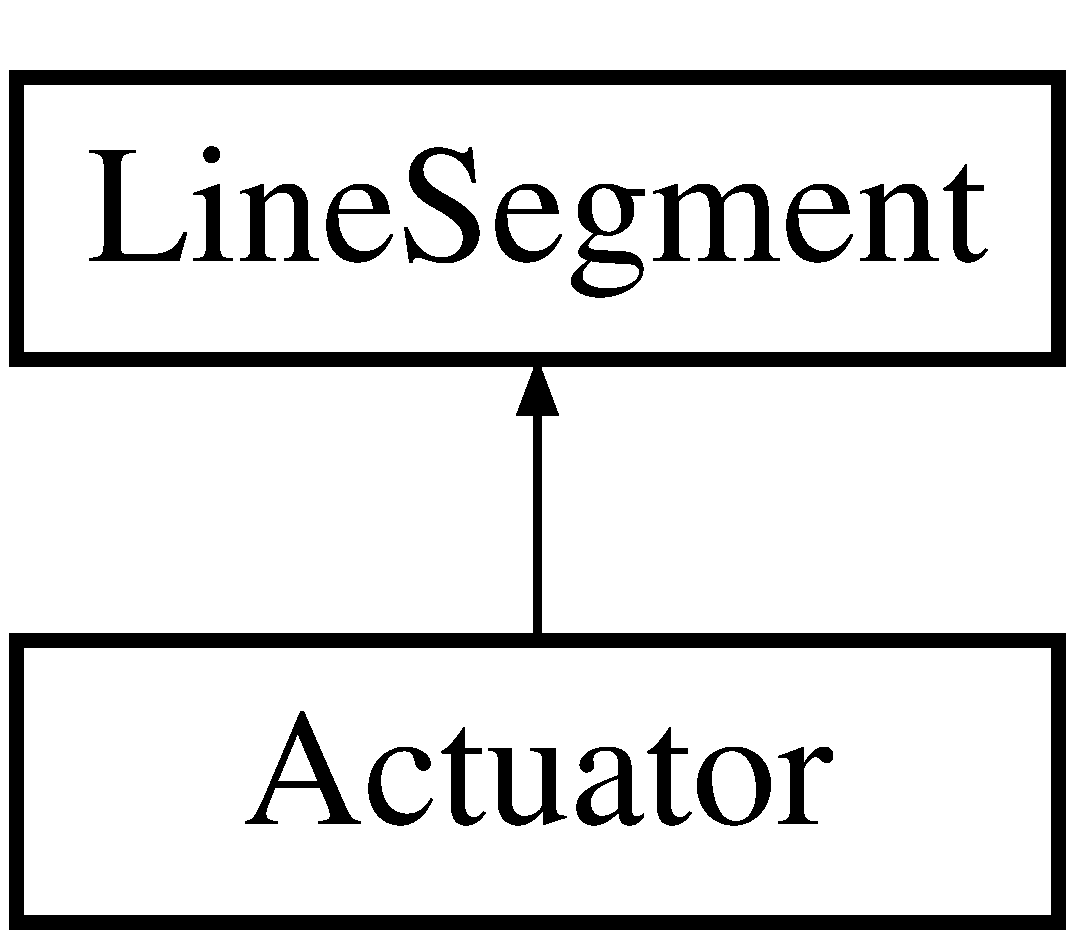
\includegraphics[height=2cm]{class_actuator}
\end{center}
\end{figure}


\subsection{Detailed Description}


Definition at line 3 of file Actuator.h.

The documentation for this class was generated from the following files:\begin{DoxyCompactItemize}
\item 
BV\_\-Creator/Actuator.h\item 
BV\_\-Creator/Actuator.cpp\end{DoxyCompactItemize}

\hypertarget{class_controller}{
\section{Controller Class Reference}
\label{class_controller}\index{Controller@{Controller}}
}
\subsection*{Public Member Functions}
\begin{DoxyCompactItemize}
\item 
\hypertarget{class_controller_ad535ad74055e645b7f44b7feeb4e82a8}{
void {\bfseries start} ()}
\label{class_controller_ad535ad74055e645b7f44b7feeb4e82a8}

\item 
\hypertarget{class_controller_ae0f9dec048daf5dfdd42b82072ac6185}{
void {\bfseries save} ()}
\label{class_controller_ae0f9dec048daf5dfdd42b82072ac6185}

\end{DoxyCompactItemize}


\subsection{Detailed Description}


Definition at line 10 of file Controller.h.

The documentation for this class was generated from the following files:\begin{DoxyCompactItemize}
\item 
BV\_\-Creator/Controller.h\item 
BV\_\-Creator/Controller.cpp\item 
BV\_\-Creator/Main.cpp\end{DoxyCompactItemize}

\hypertarget{class_environment_draw_window}{
\section{EnvironmentDrawWindow Class Reference}
\label{class_environment_draw_window}\index{EnvironmentDrawWindow@{EnvironmentDrawWindow}}
}
\subsection*{Public Member Functions}
\begin{DoxyCompactItemize}
\item 
\hypertarget{class_environment_draw_window_a89c0071b59b2f0bd92d3af3daa3281ae}{
void {\bfseries drawGrid} ()}
\label{class_environment_draw_window_a89c0071b59b2f0bd92d3af3daa3281ae}

\item 
\hypertarget{class_environment_draw_window_a20d7841b6c7b3441c1a4a418118960b2}{
int {\bfseries handle} (int event)}
\label{class_environment_draw_window_a20d7841b6c7b3441c1a4a418118960b2}

\item 
\hypertarget{class_environment_draw_window_a197a0405a52be37979e9f2fd840d25b2}{
int {\bfseries normalizeX} (int x)}
\label{class_environment_draw_window_a197a0405a52be37979e9f2fd840d25b2}

\item 
\hypertarget{class_environment_draw_window_a4ad94d20c389f3c6fefd4b5e63d97948}{
int {\bfseries normalizeY} (int y)}
\label{class_environment_draw_window_a4ad94d20c389f3c6fefd4b5e63d97948}

\item 
\hypertarget{class_environment_draw_window_a78fff980cb76a820b70c2e430a5a8322}{
void {\bfseries draw} (void)}
\label{class_environment_draw_window_a78fff980cb76a820b70c2e430a5a8322}

\item 
\hypertarget{class_environment_draw_window_a8f6cc793cd6596d26487f1f726c3d258}{
void {\bfseries save} (string filename)}
\label{class_environment_draw_window_a8f6cc793cd6596d26487f1f726c3d258}

\item 
\hypertarget{class_environment_draw_window_a9440ab68b6cc93153b0efdc8202c3eb8}{
{\bfseries EnvironmentDrawWindow} (\hyperlink{class_controller}{Controller} m, int x, int y, int w, int h, const char $\ast$lab=0)}
\label{class_environment_draw_window_a9440ab68b6cc93153b0efdc8202c3eb8}

\end{DoxyCompactItemize}
\subsection*{Public Attributes}
\begin{DoxyCompactItemize}
\item 
\hypertarget{class_environment_draw_window_a7be155615ad8160c0e5b7d7a693e6131}{
vector$<$ \hyperlink{class_point2_d}{Point2D} $>$ {\bfseries snapPoints}}
\label{class_environment_draw_window_a7be155615ad8160c0e5b7d7a693e6131}

\item 
\hypertarget{class_environment_draw_window_a09b9426601a9edcb077c5680ae83ccb3}{
vector$<$ \hyperlink{class_shape}{Shape} $>$ {\bfseries shapes}}
\label{class_environment_draw_window_a09b9426601a9edcb077c5680ae83ccb3}

\item 
\hypertarget{class_environment_draw_window_ab6cd8499bf875de0324f6c989170a39e}{
int {\bfseries MouseX}}
\label{class_environment_draw_window_ab6cd8499bf875de0324f6c989170a39e}

\item 
\hypertarget{class_environment_draw_window_a980518f83562aba40e46addb6f876e34}{
int {\bfseries MouseY}}
\label{class_environment_draw_window_a980518f83562aba40e46addb6f876e34}

\item 
\hypertarget{class_environment_draw_window_a0dc5c749f8d384ce3f73e731a5dbb6e7}{
int {\bfseries xPos}}
\label{class_environment_draw_window_a0dc5c749f8d384ce3f73e731a5dbb6e7}

\item 
\hypertarget{class_environment_draw_window_a5f90de013e245142acd042075ba18b0d}{
int {\bfseries yPos}}
\label{class_environment_draw_window_a5f90de013e245142acd042075ba18b0d}

\item 
\hypertarget{class_environment_draw_window_a9a6fa9570639af000e2a2eeabe6061e4}{
int {\bfseries wPos}}
\label{class_environment_draw_window_a9a6fa9570639af000e2a2eeabe6061e4}

\item 
\hypertarget{class_environment_draw_window_ae9de064d2c7d8e06bcc90f14b3b5ac77}{
int {\bfseries hPos}}
\label{class_environment_draw_window_ae9de064d2c7d8e06bcc90f14b3b5ac77}

\item 
\hypertarget{class_environment_draw_window_ae3fa99c93d0534b7494904389468e6e4}{
int {\bfseries size}}
\label{class_environment_draw_window_ae3fa99c93d0534b7494904389468e6e4}

\item 
\hypertarget{class_environment_draw_window_a5e1e864e0b7f6431630c576beed17e05}{
int {\bfseries margin}}
\label{class_environment_draw_window_a5e1e864e0b7f6431630c576beed17e05}

\item 
\hypertarget{class_environment_draw_window_a5d77ee07fb05b53f388648cb670357bc}{
bool {\bfseries dragging}}
\label{class_environment_draw_window_a5d77ee07fb05b53f388648cb670357bc}

\item 
\hypertarget{class_environment_draw_window_ae83da2bb35dc148f3560c2abb46b2f02}{
string {\bfseries placing}}
\label{class_environment_draw_window_ae83da2bb35dc148f3560c2abb46b2f02}

\item 
\hypertarget{class_environment_draw_window_a72981cacd507c87d5e6ba52da545135b}{
string {\bfseries nextFileName}}
\label{class_environment_draw_window_a72981cacd507c87d5e6ba52da545135b}

\item 
\hypertarget{class_environment_draw_window_a4d314332c42e568c5178adb0ef6d44ad}{
bool {\bfseries connecting}}
\label{class_environment_draw_window_a4d314332c42e568c5178adb0ef6d44ad}

\end{DoxyCompactItemize}


\subsection{Detailed Description}


Definition at line 9 of file EnvironmentDrawWindow.h.

The documentation for this class was generated from the following files:\begin{DoxyCompactItemize}
\item 
BV\_\-Creator/EnvironmentDrawWindow.h\item 
BV\_\-Creator/EnvironmentDrawWindow.cpp\end{DoxyCompactItemize}

\hypertarget{class_file_chooser}{
\section{FileChooser Class Reference}
\label{class_file_chooser}\index{FileChooser@{FileChooser}}
}
\subsection*{Public Member Functions}
\begin{DoxyCompactItemize}
\item 
\hypertarget{class_file_chooser_ade59be41e3d6d328e544289ae32f0c87}{
string {\bfseries chooseFile} (int type, string filter, string name)}
\label{class_file_chooser_ade59be41e3d6d328e544289ae32f0c87}

\end{DoxyCompactItemize}


\subsection{Detailed Description}


Definition at line 5 of file FileChooser.h.

The documentation for this class was generated from the following files:\begin{DoxyCompactItemize}
\item 
BV\_\-Creator/FileChooser.h\item 
BV\_\-Creator/FileChooser.cpp\end{DoxyCompactItemize}

\hypertarget{class_line_segment}{
\section{LineSegment Class Reference}
\label{class_line_segment}\index{LineSegment@{LineSegment}}
}
Inheritance diagram for LineSegment::\begin{figure}[H]
\begin{center}
\leavevmode
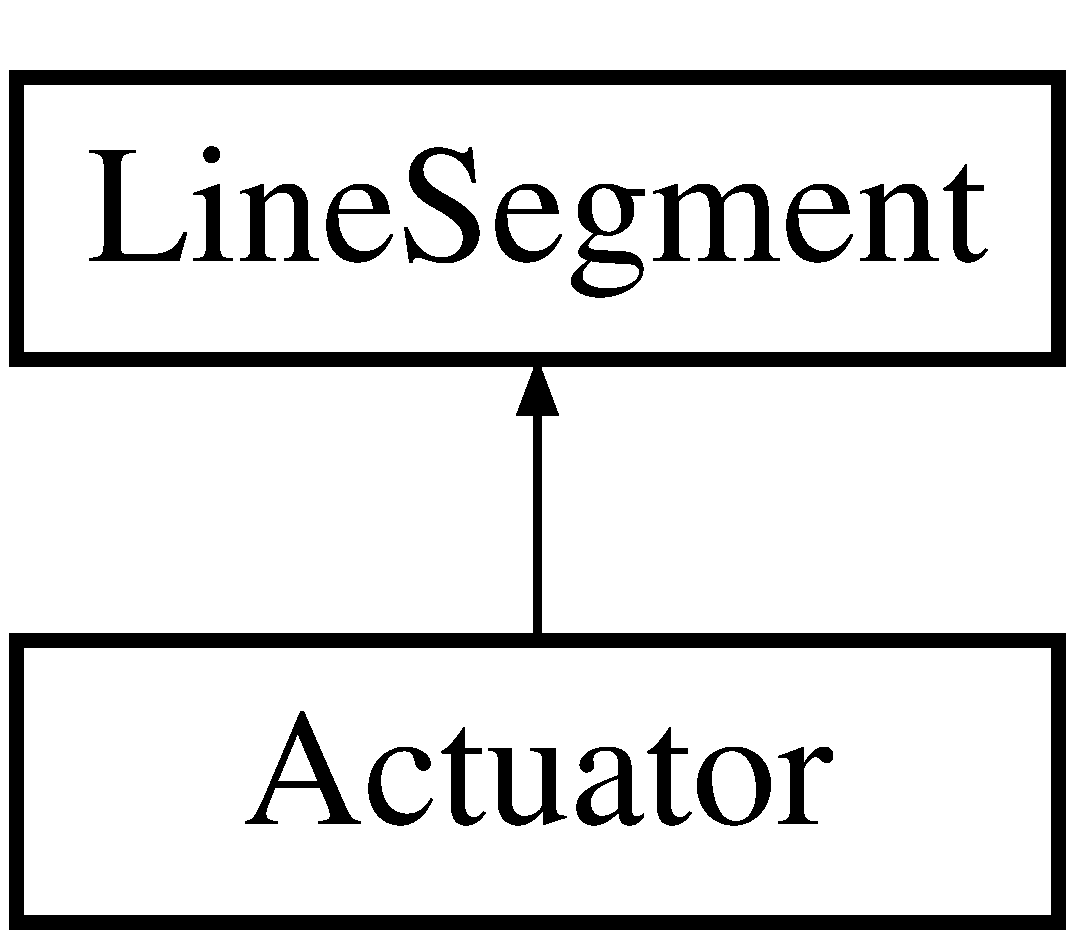
\includegraphics[height=2cm]{class_line_segment}
\end{center}
\end{figure}
\subsection*{Public Member Functions}
\begin{DoxyCompactItemize}
\item 
\hypertarget{class_line_segment_aabdfa2bc55cecfe681fe824164f7ffc0}{
void {\bfseries setx1} (int X1)}
\label{class_line_segment_aabdfa2bc55cecfe681fe824164f7ffc0}

\item 
\hypertarget{class_line_segment_a0ff3ceeb0fe95f39c28dfbfd1a0bb05a}{
void {\bfseries setx2} (int X2)}
\label{class_line_segment_a0ff3ceeb0fe95f39c28dfbfd1a0bb05a}

\item 
\hypertarget{class_line_segment_a337d14221f23e9a2dbbb020006097d22}{
void {\bfseries sety1} (int Y1)}
\label{class_line_segment_a337d14221f23e9a2dbbb020006097d22}

\item 
\hypertarget{class_line_segment_a54f151198646da740a39acb7cfc88d37}{
void {\bfseries sety2} (int Y2)}
\label{class_line_segment_a54f151198646da740a39acb7cfc88d37}

\item 
\hypertarget{class_line_segment_a89a7f2edb01d8f7e25640bf26c161d6a}{
int {\bfseries getx1} ()}
\label{class_line_segment_a89a7f2edb01d8f7e25640bf26c161d6a}

\item 
\hypertarget{class_line_segment_a8339d5ab25c7dff940e8eb77dae3720a}{
int {\bfseries getx2} ()}
\label{class_line_segment_a8339d5ab25c7dff940e8eb77dae3720a}

\item 
\hypertarget{class_line_segment_aa8ffd38d8b530bf6235dcc55914a5318}{
int {\bfseries gety1} ()}
\label{class_line_segment_aa8ffd38d8b530bf6235dcc55914a5318}

\item 
\hypertarget{class_line_segment_a65a169be88e69c3e6f8348c6b378da5f}{
int {\bfseries gety2} ()}
\label{class_line_segment_a65a169be88e69c3e6f8348c6b378da5f}

\item 
\hypertarget{class_line_segment_a3a103953d3bac4b55754f69871f7001e}{
{\bfseries LineSegment} (int X1, int X2, int Y1, int Y2, int NumberOne, int NumberTwo)}
\label{class_line_segment_a3a103953d3bac4b55754f69871f7001e}

\end{DoxyCompactItemize}
\subsection*{Public Attributes}
\begin{DoxyCompactItemize}
\item 
\hypertarget{class_line_segment_aa2034e1e99b7afc656499327c3361aee}{
int {\bfseries pointNumberOne}}
\label{class_line_segment_aa2034e1e99b7afc656499327c3361aee}

\item 
\hypertarget{class_line_segment_a66c9038a6e33eefbe7dedc95331bda72}{
int {\bfseries pointNumberTwo}}
\label{class_line_segment_a66c9038a6e33eefbe7dedc95331bda72}

\end{DoxyCompactItemize}


\subsection{Detailed Description}


Definition at line 2 of file LineSegment.h.

The documentation for this class was generated from the following files:\begin{DoxyCompactItemize}
\item 
BV\_\-Creator/LineSegment.h\item 
BV\_\-Creator/LineSegment.cpp\end{DoxyCompactItemize}

\hypertarget{class_point2_d}{
\section{Point2D Class Reference}
\label{class_point2_d}\index{Point2D@{Point2D}}
}
\subsection*{Public Member Functions}
\begin{DoxyCompactItemize}
\item 
\hypertarget{class_point2_d_ae02be3bb686d11b9bf6a0efba1ac0025}{
{\bfseries Point2D} (int X, int Y, int Color, int d, int number)}
\label{class_point2_d_ae02be3bb686d11b9bf6a0efba1ac0025}

\item 
\hypertarget{class_point2_d_a1218e9394785d0bcda3bd3823c0eb76e}{
void {\bfseries setX} (int X)}
\label{class_point2_d_a1218e9394785d0bcda3bd3823c0eb76e}

\item 
\hypertarget{class_point2_d_af34e800a83909ebc304c1433d9cf17e6}{
void {\bfseries setY} (int Y)}
\label{class_point2_d_af34e800a83909ebc304c1433d9cf17e6}

\item 
\hypertarget{class_point2_d_ac626261c1faff6d87b3dcfacac8df39e}{
void {\bfseries setColor} (int Color)}
\label{class_point2_d_ac626261c1faff6d87b3dcfacac8df39e}

\item 
\hypertarget{class_point2_d_a0e533717fefd5ee19e24eb8027c6ef00}{
void {\bfseries setDirection} (int d)}
\label{class_point2_d_a0e533717fefd5ee19e24eb8027c6ef00}

\item 
\hypertarget{class_point2_d_a558f484d3feb2432350e3d3149e72e8c}{
int {\bfseries getX} ()}
\label{class_point2_d_a558f484d3feb2432350e3d3149e72e8c}

\item 
\hypertarget{class_point2_d_a86630685042226ef670949d164ced5ca}{
int {\bfseries getY} ()}
\label{class_point2_d_a86630685042226ef670949d164ced5ca}

\item 
\hypertarget{class_point2_d_aa9d9c376b0e577e571a29d0b86201b68}{
int {\bfseries getColor} ()}
\label{class_point2_d_aa9d9c376b0e577e571a29d0b86201b68}

\item 
\hypertarget{class_point2_d_a9ccae45a94532e559e3522b74dfafcd6}{
int {\bfseries getDirection} ()}
\label{class_point2_d_a9ccae45a94532e559e3522b74dfafcd6}

\end{DoxyCompactItemize}
\subsection*{Public Attributes}
\begin{DoxyCompactItemize}
\item 
\hypertarget{class_point2_d_a02041472ec3f1ec4d92a926bad5fe2c2}{
int {\bfseries x}}
\label{class_point2_d_a02041472ec3f1ec4d92a926bad5fe2c2}

\item 
\hypertarget{class_point2_d_adbb040f0e224303093e783dfcccd4886}{
int {\bfseries y}}
\label{class_point2_d_adbb040f0e224303093e783dfcccd4886}

\item 
\hypertarget{class_point2_d_aec1d8c7b6fd28a7b4b6e22228e122216}{
int {\bfseries color}}
\label{class_point2_d_aec1d8c7b6fd28a7b4b6e22228e122216}

\item 
\hypertarget{class_point2_d_a85ac869e635bff24b324e593147f2d2a}{
int {\bfseries direction}}
\label{class_point2_d_a85ac869e635bff24b324e593147f2d2a}

\item 
\hypertarget{class_point2_d_af33232f4fa2983b4964578ea6ef445fb}{
int {\bfseries pointNumber}}
\label{class_point2_d_af33232f4fa2983b4964578ea6ef445fb}

\end{DoxyCompactItemize}


\subsection{Detailed Description}


Definition at line 2 of file Point2D.h.

The documentation for this class was generated from the following files:\begin{DoxyCompactItemize}
\item 
BV\_\-Creator/Point2D.h\item 
BV\_\-Creator/Point2D.cpp\end{DoxyCompactItemize}

\hypertarget{class_shape}{
\section{Shape Class Reference}
\label{class_shape}\index{Shape@{Shape}}
}
\subsection*{Public Member Functions}
\begin{DoxyCompactItemize}
\item 
\hypertarget{class_shape_a3b8f9a882e53fcf1852109b30fa5b75a}{
vector$<$ \hyperlink{class_line_segment}{LineSegment} $>$ {\bfseries getShape} ()}
\label{class_shape_a3b8f9a882e53fcf1852109b30fa5b75a}

\item 
\hypertarget{class_shape_a8a725902cfbe4e9dc82a1a07595ea253}{
{\bfseries Shape} (vector$<$ \hyperlink{class_line_segment}{LineSegment} $>$ s, \hyperlink{class_point2_d}{Point2D} point, string n)}
\label{class_shape_a8a725902cfbe4e9dc82a1a07595ea253}

\item 
\hypertarget{class_shape_a5dfa6164561614acd68f9dae2b2cbdf9}{
{\bfseries Shape} (\hyperlink{class_point2_d}{Point2D} point, string name, string file)}
\label{class_shape_a5dfa6164561614acd68f9dae2b2cbdf9}

\item 
\hypertarget{class_shape_a41b5e1410049bc5f4abbe1bc9df03663}{
int {\bfseries getPointNumber} ()}
\label{class_shape_a41b5e1410049bc5f4abbe1bc9df03663}

\end{DoxyCompactItemize}
\subsection*{Public Attributes}
\begin{DoxyCompactItemize}
\item 
\hypertarget{class_shape_a6adf5b999171efe7d1d122e557067106}{
\hyperlink{class_point2_d}{Point2D} {\bfseries location}}
\label{class_shape_a6adf5b999171efe7d1d122e557067106}

\item 
\hypertarget{class_shape_a05b6e95f16abf76ad3d5ae05c8ccb3c7}{
vector$<$ \hyperlink{class_line_segment}{LineSegment} $>$ {\bfseries shape}}
\label{class_shape_a05b6e95f16abf76ad3d5ae05c8ccb3c7}

\item 
\hypertarget{class_shape_afef5e9426226fd7af49fe48ec16b97f3}{
string {\bfseries name}}
\label{class_shape_afef5e9426226fd7af49fe48ec16b97f3}

\item 
\hypertarget{class_shape_a0c594b8c4dbb8c3600f9ac1f6b6a1b4a}{
string {\bfseries fileName}}
\label{class_shape_a0c594b8c4dbb8c3600f9ac1f6b6a1b4a}

\end{DoxyCompactItemize}


\subsection{Detailed Description}


Definition at line 8 of file Shape.h.

The documentation for this class was generated from the following files:\begin{DoxyCompactItemize}
\item 
BV\_\-Creator/Shape.h\item 
BV\_\-Creator/Shape.cpp\end{DoxyCompactItemize}

\hypertarget{class_vehicle_draw_window}{
\section{VehicleDrawWindow Class Reference}
\label{class_vehicle_draw_window}\index{VehicleDrawWindow@{VehicleDrawWindow}}
}
\subsection*{Public Member Functions}
\begin{DoxyCompactItemize}
\item 
\hypertarget{class_vehicle_draw_window_a16f362e2818e2221cf2b7ff5a7e5ddbc}{
int {\bfseries handle} (int event)}
\label{class_vehicle_draw_window_a16f362e2818e2221cf2b7ff5a7e5ddbc}

\item 
\hypertarget{class_vehicle_draw_window_a7f1d262d0069129e66c3d8e298338d6b}{
void {\bfseries draw} (void)}
\label{class_vehicle_draw_window_a7f1d262d0069129e66c3d8e298338d6b}

\item 
\hypertarget{class_vehicle_draw_window_ab86c94afd868ced54bf2f19144595167}{
void {\bfseries addVertPoints} (int xStart, int yStart, int yTick, int side)}
\label{class_vehicle_draw_window_ab86c94afd868ced54bf2f19144595167}

\item 
\hypertarget{class_vehicle_draw_window_a6a610ecca4517049cf1dde251e77b51d}{
void {\bfseries addHorizPoints} (int xStart, int yStart, int xTick, int side)}
\label{class_vehicle_draw_window_a6a610ecca4517049cf1dde251e77b51d}

\item 
\hypertarget{class_vehicle_draw_window_ab59fb4475a32d6eaf391661f2a1ad538}{
int {\bfseries checkPoint} (int pointX, int pointY)}
\label{class_vehicle_draw_window_ab59fb4475a32d6eaf391661f2a1ad538}

\item 
\hypertarget{class_vehicle_draw_window_a05ee2cbcfe49062f69133153792bda99}{
bool {\bfseries inMargin} (int point1, int point2, int pointMargin)}
\label{class_vehicle_draw_window_a05ee2cbcfe49062f69133153792bda99}

\item 
\hypertarget{class_vehicle_draw_window_a57ce251228aeccb7f57a9586232f59b1}{
void {\bfseries drawPoints} (vector$<$ \hyperlink{class_point2_d}{Point2D} $>$ points)}
\label{class_vehicle_draw_window_a57ce251228aeccb7f57a9586232f59b1}

\item 
\hypertarget{class_vehicle_draw_window_ab62153c6478650e51dcbe8b28370af67}{
void {\bfseries resetPoints} (vector$<$ \hyperlink{class_point2_d}{Point2D} $>$ \&points)}
\label{class_vehicle_draw_window_ab62153c6478650e51dcbe8b28370af67}

\item 
\hypertarget{class_vehicle_draw_window_abcb51594f66cbc571caa4749e309aec0}{
{\bfseries VehicleDrawWindow} (\hyperlink{class_controller}{Controller} m, int x, int y, int w, int h, const char $\ast$lab=0)}
\label{class_vehicle_draw_window_abcb51594f66cbc571caa4749e309aec0}

\item 
\hypertarget{class_vehicle_draw_window_ac334e1b40e59aea35538368db64f08ef}{
void {\bfseries addShape} (\hyperlink{class_point2_d}{Point2D} p)}
\label{class_vehicle_draw_window_ac334e1b40e59aea35538368db64f08ef}

\end{DoxyCompactItemize}
\subsection*{Public Attributes}
\begin{DoxyCompactItemize}
\item 
\hypertarget{class_vehicle_draw_window_a048b310ddc02d009da5cf159d858154f}{
vector$<$ \hyperlink{class_point2_d}{Point2D} $>$ {\bfseries snapPoints}}
\label{class_vehicle_draw_window_a048b310ddc02d009da5cf159d858154f}

\item 
\hypertarget{class_vehicle_draw_window_a805cf01d0d6a529db52b68411c4719d7}{
vector$<$ \hyperlink{class_shape}{Shape} $>$ {\bfseries shapes}}
\label{class_vehicle_draw_window_a805cf01d0d6a529db52b68411c4719d7}

\item 
\hypertarget{class_vehicle_draw_window_a9165d7ac6c2947bb13741a33183f5040}{
string {\bfseries currentShape}}
\label{class_vehicle_draw_window_a9165d7ac6c2947bb13741a33183f5040}

\item 
\hypertarget{class_vehicle_draw_window_a491adf7c5b2e88a597c941650c42a913}{
int {\bfseries MouseX}}
\label{class_vehicle_draw_window_a491adf7c5b2e88a597c941650c42a913}

\item 
\hypertarget{class_vehicle_draw_window_a965a42276f9e7e0e8ecd871a3c8eb36b}{
int {\bfseries MouseY}}
\label{class_vehicle_draw_window_a965a42276f9e7e0e8ecd871a3c8eb36b}

\item 
\hypertarget{class_vehicle_draw_window_ad1ba02b3a8e8ca0866ae46c0f412d8c8}{
int {\bfseries xPos}}
\label{class_vehicle_draw_window_ad1ba02b3a8e8ca0866ae46c0f412d8c8}

\item 
\hypertarget{class_vehicle_draw_window_a4220591c89a2654fa68ff6ae22a187a7}{
int {\bfseries yPos}}
\label{class_vehicle_draw_window_a4220591c89a2654fa68ff6ae22a187a7}

\item 
\hypertarget{class_vehicle_draw_window_a1c8ae93609082acdd686b0fbcad110fc}{
int {\bfseries wPos}}
\label{class_vehicle_draw_window_a1c8ae93609082acdd686b0fbcad110fc}

\item 
\hypertarget{class_vehicle_draw_window_ae1375d009aa87db616d3f60757e673b3}{
int {\bfseries hPos}}
\label{class_vehicle_draw_window_ae1375d009aa87db616d3f60757e673b3}

\item 
\hypertarget{class_vehicle_draw_window_a8aa5f11d4995491d9f3e192a9ce5e07d}{
int {\bfseries size}}
\label{class_vehicle_draw_window_a8aa5f11d4995491d9f3e192a9ce5e07d}

\item 
\hypertarget{class_vehicle_draw_window_a6e87d5d5b306ab3aef8e1bb703d1c58a}{
int {\bfseries margin}}
\label{class_vehicle_draw_window_a6e87d5d5b306ab3aef8e1bb703d1c58a}

\item 
\hypertarget{class_vehicle_draw_window_a73bb691b1db87413fe1c9c48ad2b9ec4}{
bool {\bfseries dragging}}
\label{class_vehicle_draw_window_a73bb691b1db87413fe1c9c48ad2b9ec4}

\item 
\hypertarget{class_vehicle_draw_window_a80c21a9690c218574fd9a7573b98b9c4}{
bool {\bfseries connecting}}
\label{class_vehicle_draw_window_a80c21a9690c218574fd9a7573b98b9c4}

\item 
\hypertarget{class_vehicle_draw_window_a182d85618993c60a8c8e210a77f3d9e8}{
bool {\bfseries notConnector}}
\label{class_vehicle_draw_window_a182d85618993c60a8c8e210a77f3d9e8}

\item 
\hypertarget{class_vehicle_draw_window_a41fcaecdbd71b3bed74293ee16075d2c}{
bool {\bfseries firstPoint}}
\label{class_vehicle_draw_window_a41fcaecdbd71b3bed74293ee16075d2c}

\item 
\hypertarget{class_vehicle_draw_window_acd8eaed08dfc9a6f0acba18b475dc86b}{
\hyperlink{class_point2_d}{Point2D} {\bfseries prevPoint}}
\label{class_vehicle_draw_window_acd8eaed08dfc9a6f0acba18b475dc86b}

\item 
\hypertarget{class_vehicle_draw_window_adb1380badfaf1aa5be9655cb39e162f7}{
int {\bfseries pointNumber}}
\label{class_vehicle_draw_window_adb1380badfaf1aa5be9655cb39e162f7}

\item 
\hypertarget{class_vehicle_draw_window_afa799f9987dc28c316d333e329e3c204}{
string {\bfseries placing}}
\label{class_vehicle_draw_window_afa799f9987dc28c316d333e329e3c204}

\item 
\hypertarget{class_vehicle_draw_window_a40cd7754a519b53686c81296dc3eff5a}{
int {\bfseries radius}}
\label{class_vehicle_draw_window_a40cd7754a519b53686c81296dc3eff5a}

\item 
\hypertarget{class_vehicle_draw_window_a3b825be21fdb11fc9985bee83bd04a2a}{
string {\bfseries file}}
\label{class_vehicle_draw_window_a3b825be21fdb11fc9985bee83bd04a2a}

\item 
\hypertarget{class_vehicle_draw_window_a0dcac62fea213a430531baac1c4fe8ec}{
int {\bfseries numPoints}}
\label{class_vehicle_draw_window_a0dcac62fea213a430531baac1c4fe8ec}

\end{DoxyCompactItemize}


\subsection{Detailed Description}


Definition at line 23 of file VehicleDrawWindow.h.

The documentation for this class was generated from the following files:\begin{DoxyCompactItemize}
\item 
BV\_\-Creator/VehicleDrawWindow.h\item 
BV\_\-Creator/VehicleDrawWindow.cpp\end{DoxyCompactItemize}

\hypertarget{class_vehicle_model}{
\section{VehicleModel Class Reference}
\label{class_vehicle_model}\index{VehicleModel@{VehicleModel}}
}
\subsection*{Public Member Functions}
\begin{DoxyCompactItemize}
\item 
\hypertarget{class_vehicle_model_ab49b0b47538cff81d3c799c63cf5e975}{
void {\bfseries save} (vector$<$ \hyperlink{class_shape}{Shape} $>$ shapes, string filename, const char $\ast$name)}
\label{class_vehicle_model_ab49b0b47538cff81d3c799c63cf5e975}

\item 
\hypertarget{class_vehicle_model_ace8af483d51893c15b4f302578e2667e}{
void {\bfseries load} (\hyperlink{class_vehicle_draw_window}{VehicleDrawWindow} $\ast$view, string filename)}
\label{class_vehicle_model_ace8af483d51893c15b4f302578e2667e}

\end{DoxyCompactItemize}


\subsection{Detailed Description}


Definition at line 20 of file VehicleModel.h.

The documentation for this class was generated from the following files:\begin{DoxyCompactItemize}
\item 
BV\_\-Creator/VehicleModel.h\item 
BV\_\-Creator/VehicleModel.cpp\end{DoxyCompactItemize}

\printindex
\end{document}
